% Convenience flattened source. Compile with XeLaTeX and the complete archive's paper/figures/ beside it.
% SPDX-License-Identifier: Apache-2.0
\documentclass[11pt,a4paper]{article}
\usepackage[margin=23mm,headheight=15pt,footskip=12mm]{geometry}
\usepackage{fontspec}
\setmainfont{P052-Roman.otf}[BoldFont=P052-Bold.otf,ItalicFont=P052-Italic.otf,BoldItalicFont=P052-BoldItalic.otf]
\setsansfont{NimbusSans-Regular.otf}[BoldFont=NimbusSans-Bold.otf,ItalicFont=NimbusSans-Italic.otf,BoldItalicFont=NimbusSans-BoldItalic.otf]
\setmonofont[Scale=0.82]{DejaVu Sans Mono}
\usepackage{amsmath,amssymb,amsthm,mathtools}
\usepackage{graphicx,booktabs,tabularx,longtable,array,multirow}
\usepackage[table]{xcolor}
\usepackage{tikz}
\usetikzlibrary{calc,arrows.meta,positioning}
\usepackage[most]{tcolorbox}
\usepackage{enumitem,microtype,titlesec,fancyhdr,caption}
\usepackage{placeins}
\usepackage[round,authoryear]{natbib}
\usepackage{xurl}
\usepackage[colorlinks=true,linkcolor=Plum,citecolor=Plum,urlcolor=Plum,breaklinks=true]{hyperref}
\definecolor{Ink}{HTML}{151326}
\definecolor{Plum}{HTML}{5530A0}
\definecolor{Violet}{HTML}{B69BFF}
\definecolor{Mint}{HTML}{8FE4D0}
\definecolor{Gold}{HTML}{E7C889}
\definecolor{Mist}{HTML}{F3F0FA}
\definecolor{Slate}{HTML}{5A566A}
\definecolor{Line}{HTML}{D8D1E7}
\hypersetup{pdftitle={AGI ALPHA: The Advantage You Can Build},pdfauthor={MONTREAL.AI},
 pdfsubject={Constructive Foresight for the Intelligence Transition},pdfkeywords={constructive foresight,readiness,mission alpha,value of information,calibration,TI,scientific computing},pdfcreator={XeLaTeX}}
\color{Ink}
\setlength{\parskip}{5pt}
\setlength{\parindent}{0pt}
\setlength{\emergencystretch}{2em}
\widowpenalty=10000
\clubpenalty=10000
\displaywidowpenalty=10000
\brokenpenalty=10000
\raggedbottom
\renewcommand{\arraystretch}{1.16}
\titleformat{\section}{\Large\sffamily\bfseries\color{Plum}}{\thesection}{0.7em}{}
\titleformat{\subsection}{\large\sffamily\bfseries\color{Ink}}{\thesubsection}{0.7em}{}
\titleformat{\subsubsection}{\normalsize\sffamily\bfseries}{\thesubsubsection}{0.7em}{}
\titlespacing*{\section}{0pt}{16pt}{7pt}
\titlespacing*{\subsection}{0pt}{11pt}{5pt}
\setlist{nosep,leftmargin=1.5em,topsep=5pt}
\captionsetup{font=small,labelfont={bf,sf},textfont=normalfont,skip=7pt}
\newcolumntype{Y}{>{\raggedright\arraybackslash}X}
\newcolumntype{L}[1]{>{\raggedright\arraybackslash}p{#1}}
\pagestyle{fancy}
\fancyhf{}
\fancyhead[L]{\sffamily\scriptsize\color{Slate}AGI ALPHA}
\fancyhead[R]{\sffamily\scriptsize\color{Slate}CONSTRUCTIVE FORESIGHT}
\fancyfoot[L]{\sffamily\scriptsize\color{Slate}MONTREAL.AI \quad Research edition 1.0}
\fancyfoot[R]{\sffamily\small\thepage}
\renewcommand{\headrulewidth}{0.3pt}
\newtcolorbox{claimbox}[1][]{colback=Mist,colframe=Line,colbacktitle=Plum,coltitle=white,boxrule=0.5pt,arc=2mm,left=4mm,right=4mm,top=3mm,bottom=3mm,#1}
\newcommand{\TI}{\ensuremath{\mathrm{TI}_{\infty}}}
\newcommand{\MA}{\ensuremath{\Delta V_{\mathrm{mission}}}}
\newcommand{\obs}{\textsf{Observed}}
\newcommand{\simu}{\textsf{Simulated}}
\newcommand{\assum}{\textsf{Assumed}}
\newcommand{\pend}{\textsf{Pending}}
\newcommand{\source}{\textsf{Source-derived}}
\newtheorem{proposition}{Proposition}
% Generated from retained results; no experiment is executed.
\newcommand{\PrimaryBrier}{0.0721}
\newcommand{\BaseBrier}{0.2600}


\begin{document}
\hypersetup{pageanchor=false}
\begin{titlepage}
\pagecolor{Ink}\color{white}\thispagestyle{empty}
\begin{tikzpicture}[remember picture,overlay]
\fill[Plum!24!Ink] ($(current page.north east)+(-4,-5)$) circle (5.0cm);
\draw[Violet!34, line width=0.6pt] ($(current page.north east)+(-3.8,-5.5)$) circle (4.25cm);
\draw[Violet!14, line width=0.5pt] ($(current page.north east)+(-3.8,-5.5)$) circle (5.1cm);
\foreach \x/\y in {2/3,6/1,13/4,3/14,17/17,8/22,16/25,1/20,10/8,18/11}{
 \fill[white,opacity=.45] ($(current page.south west)+(\x,\y)$) circle (0.45pt);}
\draw[Mint,line width=1.3pt] ($(current page.south west)+(2.3,6.8)$) .. controls +(4,0) and +(-3,-1) .. ($(current page.south west)+(12.5,9.2)$);
\draw[Gold,line width=0.8pt,dashed] ($(current page.south west)+(12.5,5.7)$)--($(current page.south west)+(12.5,10.0)$);
\fill[Mint] ($(current page.south west)+(9.6,8.2)$) circle (2.2pt);
\node[anchor=west,text=Mint,font=\sffamily\small] at ($(current page.south west)+(2.3,6.2)$) {CAPABILITY READY};
\node[anchor=west,text=Gold,font=\sffamily\small] at ($(current page.south west)+(12.7,6.0)$) {WINDOW CLOSES};
\end{tikzpicture}
{\sffamily\small\color{Mint}MONTREAL.AI \hfill RESEARCH / 09}\par
\vspace{24mm}
{\sffamily\fontsize{18}{22}\selectfont\color{Violet}AGI ALPHA}\par
\vspace{6mm}
{\sffamily\bfseries\fontsize{35}{39}\selectfont THE ADVANTAGE\\YOU CAN BUILD}\par
\vspace{9mm}
{\sffamily\fontsize{17}{23}\selectfont Constructive Foresight\\for the Intelligence Transition}\par
\vspace{11mm}
\begin{minipage}{0.77\linewidth}
{\large The future creates no advantage until something useful is ready.}\par
\vspace{4mm}
{\color{Violet}Test the forecast. Build the capability. Make readiness earn its cost.}
\end{minipage}
\vfill
{\sffamily\small TRANSFORMATIONAL INTELLIGENCE $\infty$ \quad / \quad SUCCESSOR $\Omega$}\par
\vspace{4mm}
{\small Research and engineering edition 1.0 \quad 24 October 2026 (UTC)}\par
{\scriptsize\color{Violet}Original cover schematic. It is a conceptual relationship, not a measured forecast.}
\end{titlepage}
\nopagecolor\color{Ink}
\setcounter{page}{1}
\hypersetup{pageanchor=true}

\begin{center}
{\Large\sffamily\bfseries AGI ALPHA: The Advantage You Can Build}\par
\vspace{3pt}
{\large Constructive Foresight for the Intelligence Transition}\par
\vspace{6pt}
MONTREAL.AI \quad $\cdot$ \quad Research and engineering edition 1.0
\end{center}
\section*{Abstract}
Could the intelligence transition become an extraordinary opportunity, and when does anticipating it help an agent build something useful? We define \emph{constructive foresight} as a policy that acquires decision-relevant information and prepares a qualified capability before its delivery window closes. \emph{Mission Alpha} is incremental beneficiary value after full costs relative to a credible alternative. The study separates observed numerical capability, prospective local timing forecasts, modeled adoption and unobserved commercial acceptance. A preregistered instrument on four fixed public sparse matrices passes all 432 held-out batches and 3,024 manufactured right-hand sides. Reuse is 7.0--13.6 times faster than repeated setup at 16 right-hand sides, but conventional cached factorization explains the benefit: added certification has median time ratios of 1.01--1.44 relative to that strong baseline. Frozen primary-deadline forecasts achieve Brier \PrimaryBrier{} versus \BaseBrier{} for a pooled constant, on 720 correlated local outcomes. In 4,608 paired simulated worlds, constructive foresight's nominal increment over the calibration-selected rule is $+0.0257$ assumed credits per episode (95\% seed-block interval $[-0.0389,0.1273]$); reversed signals produce a loss. A compiled conventional policy with identical information chooses the same actions throughout and costs less to run. Published Alpha, Jobs and Manager components demonstrate knowledge-only restoration, fresh proof and separate explicit authority, with 14 expected refusals retained. The result is a working readiness method and a precise negative boundary: this study does not establish a unique full-cost advantage for foresight or observed customer value. Readiness is useful only when it pays for itself against the best available response.


\begin{claimbox}
\textbf{The test.} Did foresight help build useful advantage in time, after full costs, against a credible alternative?\\[3pt]
\textbf{The evidence boundary.} Numerical execution is measured. Demand, adoption, imitation and pricing are controlled assumptions. The dispatcher demonstration uses a public test identity. No external beneficiary acceptance, settled revenue or commercial full-cost advantage is established.
\end{claimbox}
\vspace{2mm}
\textbf{Keywords:} constructive foresight; mission alpha; readiness; value of information; calibrated delivery; learning-augmented decisions; reproducible numerical instruments.

\section{From a large transition to one difficult decision}
Could a transition toward increasingly affordable machine intelligence create extraordinary opportunity? The question is reasonable, but its scale does not tell an agent what to do next. A sector can expand while a particular intervention is late, unneeded, expensive, untrusted or already available from somebody else. Predicting a change and delivering a useful response to it are different accomplishments.

This paper moves the unit of analysis from a predicted winning sector to a bounded mission. An agent must identify a beneficiary's bottleneck, decide whether more information is worth acquiring, construct a capability if justified, qualify its output, and deliver before the relevant opportunity closes. The alternative may be a conventional engineer who uses exactly the same tools. The agent can also decline construction. Waiting is a substantive action, not a missing stage in a success story.

The central object is a \emph{readiness certificate}: an inspectable connection among a frozen computational recipe, an input identity, finite capability evidence, a conditional delivery forecast, a cost ledger and a separate execution-authority boundary. It does not certify the future. It makes the assumptions that would justify preparing for that future explicit, and makes loss of those assumptions observable. Our artifact applies this object to repeated sparse linear solves. Its kernel is conventional SuperLU; the research contribution is the integrated, falsifiable decision and evidence procedure, not a new factorization algorithm.

We test three distinct propositions. First, preparation can change which numerical investigations meet a short response deadline. Second, a probabilistic forecast can be evaluated against subsequent local computation without pretending to forecast industrial adoption. Third, timing information can change a build-or-wait decision in a finite model, but a competent conventional policy with the same information may match or exceed it. All three are needed to interpret ``advantage.'' None implies that an agent has forecast AGI, discovered a new market, earned revenue or outperformed an unrestricted human organization.

\subsection{A prominent boundary around the macro scenario}
\begin{claimbox}[title={\sffamily Assumption panel: the $\$15$ quadrillion envelope}]
The project's original Living Treasure Map initializes an editable $\$15$ quadrillion envelope and a twenty-year horizon. Twelve weights distribute that assumed total. The current Insight Atlas explicitly calls its envelope a scenario assumption and reports verified economic value as zero. These controls are not measured wealth, a total addressable market, a forecast, a token valuation or a promise of investment return. This paper does not use the envelope to generate its experimental outcomes or economic verdict. \citep{atlas2026,treasure2026}
\end{claimbox}

The distinction also prevents an accounting error: multiplying an assumed envelope by an assumed capture fraction does not produce observed profit. The original twenty-year horizon is separate from the Atlas agent-firm planner's 120-minute default. Its original twelve weights and the current exact-integer fixture weights are different scenario inputs, not inconsistent estimates of a real economy. Appendix~\ref{app:macro} preserves the precise source distinction.

\subsection{What is new, and what is inherited}
\TI{} motivates executable changes in representation, information, construction and strategy, together with a bridge back to the authorized purpose and a comparison that pays transformation costs. The project already contains papers on learning, reasoning, design, strategy, execution and evolution. In particular, combining information with construction is not new to this project. \citep{ti2026,outlearn2026,outstrategise2026,outexecute2026}

Writer 9 isolates the \emph{time-dependent decision}: whether an information acquisition and capability construction finish early enough to improve qualified delivery over an equally equipped alternative. It contributes a reusable readiness implementation, a frozen prospective local-delivery ledger, a finite timing experiment, and source-bound lifecycle evidence. It does not inherit Writer 6's experimental cases or results. It is distinct from Writer 8's opportunity-ledger and capacity-investment question: no sector ranking or allocation of a macro envelope is a primary outcome here. Earlier editions remain unchanged.

\section{Prior art and the novelty boundary}
Probability forecasts require scoring rules that reward accurate probability statements. The Brier score evaluates a binary event, while strictly proper scoring rules provide a general framework for honest probabilistic assessment. \citep{brier1950,gneiting2007} A lower score is not, by itself, a better decision: forecasting quality, correspondence to observations and value to a decision maker are separable. \citep{murphy1993} Decision-aware prediction makes this dependence on the downstream optimization problem explicit. \citep{elmachtoub2022}

Value-of-information analysis evaluates an information acquisition by its effect on an explicit decision, net of acquisition costs. \citep{howard1966} The option to wait is also established: an irreversible investment under uncertainty can be inferior to postponement even when a simple expected-value calculation appears favorable. \citep{mcdonald1986} Learning-augmented online algorithms already use predictions for ski rental and scheduling. \citep{purohit2018} We therefore do not present prediction-assisted construction timing as a newly invented problem or claim competitive guarantees for our finite experimental policies.

A further complication is intervention. A forecast used to change the world is not being evaluated against the world that would have existed without that action. Performative prediction formalizes cases in which the deployed predictive procedure changes its target distribution. \citep{perdomo2020} Here, preparing a factorization changes response latency; preparation is not a successful prediction that latency would have improved unaided. We keep forecasts conditional on readiness state and distinguish no-action outcomes from preparation-conditioned outcomes.

Numerical reuse also has a substantial history. Sparse direct solvers reuse a factorization across right-hand sides, and Krylov-subspace recycling addresses related sequences of linear systems. \citep{davis2011,parks2006} Conjugate gradients is a classical method for suitable positive-definite systems. \citep{hestenes1952} We use standard numerical kernels and a fixed set of public Harwell--Boeing matrices. Small residuals are not universal forward-error guarantees, especially on ill-conditioned systems. \citep{higham2002} The acceptance criteria therefore expose both residual and manufactured-solution error rather than renaming a solver convergence flag as verification.

The contribution should be judged as a reproducible research-and-engineering integration with a discriminating experiment. It supplies neither a new sparse numerical algorithm nor a theorem that foresight invariably creates economic value. Its useful scientific outcome can be a negative comparative result: a functioning capability, a forecast with measurable skill, and no net advantage over a competent adaptive builder.

\section{Formalizing constructive foresight}
\subsection{Mission, information and policies}
A mission is the tuple
\begin{equation}
\mathcal M=(b,g,\mathcal A,\mathcal I_0,H,R,Q,U),
\end{equation}
where $b$ identifies the beneficiary, $g$ the bottleneck, $\mathcal A$ the feasible actions, $\mathcal I_0$ the initial information, $H$ the horizon, $R$ the resource constraint, $Q$ the acceptance predicate and $U$ the mission utility. A policy $\pi$ maps the information available at each decision time to a feasible action, including information acquisition, construction, reuse, waiting or abstention. Feasibility includes authority, not only technical possibility.

Let $Y^\pi_{j,H}$ indicate that output $j$ is useful, accepted and delivered by its mission deadline under policy $\pi$. Let $C^\pi$ include inference, acquisition, search, engineering, validation, human review, failed work, maintenance, execution and orchestration without double-counting. Currency expenditures and imputed time costs remain different ledger fields. Then
\begin{align}
V_H(\pi)&=U_b(Y^\pi_{1,H},\ldots,Y^\pi_{m,H})-C^\pi,\\
\MA(\pi;\pi_0)&=\mathbb E[V_H(\pi)-V_H(\pi_0)\mid\mathcal I_0].
\end{align}
\emph{Mission Alpha} is this incremental mission value relative to an eligible, credible alternative under comparable constraints. It is unrelated to a claim of financial-security alpha. A realized difference may be reported after outcomes occur; an expectation under an assumed world distribution remains a modeled quantity.

The strongest alternative is defined by the available policy class and information boundary. For this finite study, the primary comparator is selected using calibration only and locked before confirmation. We additionally report the proposed policy against every eligible alternative. A per-episode perfect-future choice is an oracle upper reference, not an eligible real-world competitor. Unknown authoring or acceptance costs prevent a claim that a computed runtime difference is a complete commercial value difference.

\subsection{A window is a joint distribution}
Write $T_B$ for construction and qualification readiness, $T_X$ for execution time, $T_Q$ for final acceptance delay, $T_A$ for adoption, $T_C$ for competitor availability, $T_I$ for imitation and $T_D$ for demand change. These can be dependent. The joint distribution matters because the same demand information that makes construction attractive may also accelerate competing supply.

For a request arriving at $t$, a conditional delivery target has the form
\begin{equation}
p_\pi(d\mid\mathcal I_t)=\Pr\!\left(Q=1,\;T^\pi_{\mathrm{delivery}}\leq d\mid\mathcal I_t\right).
\end{equation}
If the capability is already ready, $T_B$ is a sunk preparation cost and is excluded from \emph{response latency}; it is still included in the policy's \emph{total cost}. A cold-state delivery target includes the remaining preparation delay. Pooling the two would reward an unpriced change of intervention.

Competitive imitation changes the best alternative available to the beneficiary. It does not destroy the fact that a solver can save CPU time. We therefore treat competitive availability as a change in the comparison and routing options, and treat price compression as an explicitly assumed economic parameter. Scientific usefulness, exclusivity, adoption and appropriable proceeds are not interchangeable columns.

\subsection{Information has value only through a decision}
For an acquisition $Z$ costing $c_Z$ and delaying the decision by $\delta_Z$, define
\begin{equation}
\operatorname{VOI}(Z)=\mathbb E_Z\!\left[\max_{a\in\mathcal A_{t+\delta_Z}}\mathbb E[V(a)\mid\mathcal I_t,Z]\right]
-\max_{a\in\mathcal A_t}\mathbb E[V(a)\mid\mathcal I_t]-c_Z.
\end{equation}
The action set and its attainable outcomes may shrink during acquisition. A confidence score that ignores this delay is not value of information. The same calculation must be available to a credible conventional competitor; the proposed procedure does not receive free search or free measurements.

\begin{proposition}[Decision invariance]
If one feasible action maximizes expected mission value for every possible acquisition result, and the acquisition does not improve that action's implementation or feasible set, acquiring the information cannot increase expected value before cost. A positive acquisition cost strictly reduces net value.
\end{proposition}
\begin{proof}
With the same maximizing action $a^*$ in every posterior state, the law of total expectation gives $\mathbb E_Z\mathbb E[V(a^*)\mid\mathcal I_t,Z]=\mathbb E[V(a^*)\mid\mathcal I_t]$. The maximization contributes no additional term. Subtract acquisition cost, and any loss caused by its delay, to obtain the claim.
\end{proof}

This simple observation supplies a falsifier. A forecast can improve Brier score yet leave the build decision unchanged. Conversely, an imprecise forecast near a consequential threshold may be valuable. Our experimental reports retain both forecast scores and policy values, and never infer one from the other.

\section{Mission selection and the enabling instrument}
\subsection{Why this mission was selected before results}
The initial protocol examined five concrete work families before running a solver. Table~\ref{tab:missions} records the selection. The choice prioritized public inputs, finite acceptance, reproducibility and a credible baseline. It did not select the task by observed favorable effect size.

\begin{table}[ht]
\centering\small
\begin{tabularx}{\linewidth}{@{}L{28mm}YY@{}}\toprule
Work family & Observable bottleneck & Decision before execution \\\midrule
Scientific computing & Repeated setup and quality checking of linear solves & Selected: public matrices; direct acceptance and clocks. \\
Energy-system design & Qualified engineering constraints and operational context & Rejected for deep execution: no operator acceptance or operating data. \\
Research instrumentation & Physical detector calibration and access & Rejected: unavailable apparatus; avoid duplicating spectral-instrument studies. \\
Biomedical discovery & Experimental confirmation and adoption & Rejected: no biological validation or beneficiary acceptance in scope. \\
Release verification & Reproducible software qualification & Rejected as primary mission: overlaps active held integration lanes. \\\bottomrule
\end{tabularx}
\caption{\assum{} / preregistered selection judgment. These are work-family feasibility assessments, not sector forecasts or measured demand.}
\label{tab:missions}
\end{table}

The beneficiary is a numerical researcher conducting repeated public-benchmark investigations. No external researcher agreed to accept the artifact during this study. Consequently, ``accepted'' in numerical tables means the frozen computational predicate passed. It does not mean customer acceptance. The useful artifact is a source-bound, reusable solve-and-check instrument with an inspectable reconstruction recipe and honest cost measurements. We test whether it makes a specified local deadline feasible; we do not claim that the underlying linear-system class was previously unsolvable.

\subsection{Public inputs and provenance limitations}
The four fixed matrices are HB/1138\_bus, HB/bcsstk14, HB/bcsstk18 and HB/bcsstk24. They originate in power-network or structural calculations and are cataloged in the SuiteSparse Matrix Collection. \citep{davis2011,kolodziej2019} They are small enough for finite local replication and sufficiently ill-conditioned to make careless residual-only claims inappropriate. The experiment uses manufactured right-hand sides $b=Ax_\star$, with $x_\star$ sampled from a fixed standard-normal generator. These right-hand sides are synthetic; the matrix origins do not make them real operating missions.

Official file endpoints returned acquisition errors. Before any solver run, amendment A01 fixed pinned public research copies of the same four named matrices. Numeric Matrix Market payloads were preserved, transport and payload hashes recorded, and dimensions and expanded nonzero counts checked against official records. A pattern-only bcsstk14 candidate was rejected during data validation. Equality to unavailable official download bytes is \emph{not} established. The packaged data and provenance make the actual experiment reproducible despite that boundary.

The collection describes these cases as positive definite; an older NIST bcsstk24 page uses an indefinite label. Our primary SuperLU comparison does not require positive definiteness. The optional Jacobi-preconditioned conjugate-gradient run is a bounded diagnostic, not a theoretical claim covering every input. No test certifies the underlying arena, power station or power network.

\subsection{What the readiness instrument actually builds}
The instrument factorizes the exact matrix with SciPy SuperLU in float64 using COLAMD ordering, performs two fixed preflight solves with separate seed 770001, checks their outputs, and binds the recipe to matrix, numerical-source and environment hashes. \citep{scipySplu} It retains the factorization in memory for subsequent right-hand sides. Every later output is checked again. A preflight success is finite evidence of that recipe, not permission to accept all future outputs.

The exported recipe includes acceptance thresholds, solver and library versions, source and matrix identities, and an explicit absence of execution authority. Restoration reads and verifies those identities, then \emph{refactorizes and revalidates}. A recipe is not a serialized SuperLU factor. Reconstruction time is measured and charged. A stale source, changed matrix, changed environment or altered acceptance policy is rejected.

The numerical acceptance predicate is column-wise. For every right-hand side it requires finite output, relative $\ell_2$ residual at most $10^{-9}$, normwise $\ell_\infty$ backward error at most $10^{-12}$, and manufactured relative $\ell_2$ solution error at most $10^{-4}$:
\begin{align}
r_j&=\frac{\|b_j-A\hat x_j\|_2}{\|b_j\|_2}, &
\eta_j&=\frac{\|b_j-A\hat x_j\|_\infty}{\|A\|_\infty\|\hat x_j\|_\infty+\|b_j\|_\infty},\\
e_j&=\frac{\|\hat x_j-x_{\star,j}\|_2}{\|x_{\star,j}\|_2}.&&
\end{align}
A batch qualifies only if every column passes. The manufactured solution permits the forward-error check in this benchmark; a user without a known answer cannot infer the same forward-error evidence from a residual alone. This limitation is retained in the interface and paper.

\section{A preregistered, finite study}
\subsection{Registration chronology and budgets}
The initial design was written before any numerical result, saved durably and reopened with every manifest payload checked. Its SHA-256 begins \texttt{aebdfe90edf392d8}; the full identity appears in the package. The public coordination record contains the initial checkpoint identity. \citep{registration2026} A01 documents data-source changes without replacing a matrix, and A02 clarifies estimands and shared overhead. Source freezes and forecast issuance records are retained in the package.

Development uses a single fixed engineering block, with at most two retained bug-fix reruns. Calibration uses eight blocks; confirmation uses twelve later blocks. Each block covers four matrices, three right-hand-side counts ($1,4,16$), and three methods, producing 288 planned calibration and 432 planned confirmation batches. The primary numerical count is $q=16$. All confirmation predictions are issued together before opening a confirmation seed. The independent finite timing model has a separate source/configuration freeze before its own trials.

Each numerical phase has a 300-second wall budget, with a whole-study computational budget of 1,800 CPU seconds for the declared experimental runs. Budget stops retain the count of unexecuted planned cells. There is no replacement sampling, outcome-dependent stopping or expansion until a favorable matrix appears. Authoring and research-tool activity are outside this measured runtime cap and remain a separate, incompletely metered cost category.

\subsection{Competent numerical alternatives}
\textbf{Cold direct} refactorizes for each right-hand side. It shows the value of reuse but is deliberately labeled an ablation. \textbf{Native cached} uses a conventional single factorization and batched solves, with the same per-output acceptance predicate. It is the strong numerical comparator. \textbf{Certified ready} adds the source-bound recipe and two preflight checks to the same factorization algorithm. A specialist sparse Cholesky implementation was not installed; the comparison is bounded to the tested common SuperLU interface, not every possible sparse solver.

Method order is randomized within each matrix/block/count cell and BLAS thread count is fixed to one. The ledger records setup, preflight, metadata, solve, validation, other overhead, total wall time and process time. Read/hash/parse and workload-generation effort are shared campaign overhead. A contextual generation-time field repeated in result rows is never summed as if that shared work occurred once per method. Phase wall and CPU totals retain unallocated orchestration and file-writing costs.

Known historical matrices may already be familiar to language-model training. No claim of clean retrospective model forecasting is made. The local timing outcomes are produced after forecast issuance, using a deterministic numerical policy rather than an evaluating language model. Repeated right-hand sides and deadlines are correlated observations. They do not constitute independent industries or beneficiaries.

\subsection{Prospective local forecasts}
For each matrix, count, method and readiness state, the calibration data define an empirical delivery distribution. Deadline multipliers $0.5,1,2$ apply to the corresponding calibration median native-cached total time; multiplier 1 is primary. A target resolves positively only if the batch qualifies and the relevant elapsed time is at or below its frozen deadline. Cold-state targets include setup. Ready-state targets condition on both factors and manufactured right-hand sides already being available. This stage is observed inside a full-cost batch; it is not a separately observed beneficiary arrival.

With $s$ calibration successes among $n=8$ observations, the issued probability is $(s+1)/(n+2)$. A calibration-only constant base rate is an explicitly weaker reference. The freeze file contains every probability, deadline, issue time, source hash and calibration hash. It permits a fixed launch window; the actual start timestamp plus the frozen elapsed deadline determines each local event time. No probability is updated after seeing an earlier confirmation result.

We report Brier score $\frac1N\sum_i(p_i-y_i)^2$, descriptive reliability bins and per-state outcomes. Better scores relative to a pooled constant show conditional information about this narrow computational workload, not a validated forecasting method for industrial adoption. The decision experiment must separately show whether information changes actions and increases net mission utility.

\subsection{A controlled timing experiment, anchored to measured work}
Real computation cannot reveal the counterfactual demand that a different policy would have encountered. We therefore separate an observed capability trial from a controlled timing model. The model uses only numerical \emph{calibration} runtimes. It does not manufacture an observed customer, an adoption event or a day-scale industrial lead time.

One common clock unit is the median build time across the four frozen matrix primitives: 0.047096737755 seconds. The horizon is eight units. A binary forecast target asks whether at least one numerically qualified request is delivered by absolute model time four and before its expiry. The no-action alternative rents available conventional service; construction changes the delivery distribution. Forecasts are explicitly conditional on the chosen plan and its information acquisition.

Before decision calibration, the executable source and protocol fixed six regimes, eight calibration seeds (101--108), twenty-four confirmation seeds (201--224), and 32 episodes per seed per regime. A finite calibration scenario bank estimates action values and event probabilities. The training file, selected comparator, primitives, source and protocol were then hashed in a separate freeze, saved durably, reopened and publicly recorded before confirmation. Every eligible policy receives the same context, frozen model, tools, signal-purchase option and construction plans. Actual deployed policy work and model preparation are charged.

Table~\ref{tab:policies} gives the competitors. ``Expert'' is a code label for a strong calibration-optimized rule; no human expert was recruited. The fixed rule can select a plan with adaptive arrival recourse. Thus ``static'' does not mean a deliberately helpless competitor. The same-information adaptive competitor compiles the finite decision rule during preparation, and may match constructive foresight exactly.

\begin{table}[ht]\centering\small
\begin{tabularx}{\linewidth}{@{}L{35mm}Y@{}}\toprule
Policy & Allowed behavior and role \\\midrule
Forecast only & Buys the signal and rents conventional service. Construction is removed as a declared ablation. \\
Constructive foresight & Evaluates finite prior and posterior plans, acquires information only for positive modeled net VOI, then builds, rents, defers or uses arrival recourse. \\
Wait and act & Waits for observed demand and then constructs. Timing ablation; does not exploit cheap competing service. \\
Calibrated fixed rule & Selects the best prior plan from the calibration model, including adaptive arrival recourse; pays model preparation. Locked primary comparator after calibration. \\
Adaptive, no forecast & Uses observed arrival, request count, expiry and available conventional service to decide whether to build or rent. No acquired forecast. \\
Adaptive, same information & Uses the same model, signal and feasible plans as constructive foresight, compiled into a conventional decision table. Pays preparation and actual dispatch work. \\
Clairvoyant menu & Exact best realized choice among the finite common plan menu and build-at-demand with future events revealed. Nondeployable upper reference; excluded from comparator selection. \\\bottomrule
\end{tabularx}
\caption{Preregistered controlled-model design. Forecast-only and wait-and-act policies are explicit ablations. Strong competitors can construct capabilities and use the same tools. No real-world organization is represented by a measured performance claim.}
\label{tab:policies}\end{table}

The base demand probabilities are 0.10, 0.35 and 0.70. A demanded episode requests 1, 4, 16 or 64 outputs with probabilities 0.45, 0.30, 0.20 and 0.05. The declared nominal adoption probability is 0.85. Request arrival, adoption delay, expiry, competitor arrival and imitation lag are sampled from explicit finite distributions in the protocol. Information acquisition costs 0.05 clock units and also delays action. Alternative service amortizes its measured construction cost over an assumed 64 requests, available equally to all policies. That amortization is an assumption, not observed demand or free competitor capital.

\begin{table}[ht]\centering\small
\begin{tabularx}{\linewidth}{@{}L{34mm}YY@{}}\toprule
Regime & Declared change & Testable failure mechanism \\\midrule
Nominal & Signal accuracy 0.8, nominal adoption and competition & Can information change a worthwhile construction decision? \\
Uninformative signal & Known accuracy 0.5 & Does the policy avoid paying for information with no decision value? \\
Costly construction & Build cost multiplied by 8; demand probability by 0.45 & Can speculative preparation or mandatory late construction destroy value? \\
Delayed demand & Actual arrival delayed by 6 units and adoption falls to 0.45; unannounced to the model & Does outdated timing create idle capability and missed useful demand? \\
Fast imitation & Earlier competing supply and short imitation lags & Does an accessible alternative remove the reason to build privately? \\
Distribution shift & Actual signal accuracy 0.2 while the model assumes 0.8 & Does a confident but reversed signal lead to harmful intervention? \\\bottomrule
\end{tabularx}
\caption{\assum{} / \simu{}. These stress regimes are declared causal interventions inside the finite model. Their frequencies are not empirical sector base rates.}
\label{tab:regimes}\end{table}

The information boundary is strict. At arrival, the policy observes demand, count, current time, expiry and current alternative availability. Before then, it cannot see the actual future arrival, expiry, competitor times, sampled service durations or success draws. Request admission uses calibrated duration estimates. Once admitted, an attempt pays its actual sampled duration even if it finishes late. Late numerical success is not qualified on-time delivery. The clairvoyant reference is the only arm with perfect future-event knowledge, and its ideal-menu bound is reported separately from its measured search cost.

Each qualified on-time request receives one \emph{assumed} mission credit. Cost is one credit per common clock unit. Accounted seconds sum replayed numerical wall time, assumed acquisition/competitor time and measured controller/preparation CPU at that explicit common price. They are neither metered total CPU nor currency. Actual controller wall time delays dispatch; CPU measures its cost. Full model-fitting CPU is allocated to each independently deployed model-using policy over the declared 4,608 confirmation episodes, not divided among policies as a shared free resource. Study execution counts the actual fitting process once in its separate measured ledger.

Wait-and-act and adaptive-without-forecast receive offline shared-evaluator probability estimates only \emph{after} their timed decision. Those estimates are excluded from policy calibration plots and their evaluator CPU is study overhead. The oracle's zero-error retrospective event label is likewise not a forecast. Policy-conditional forecast scores use only probabilities available before the corresponding simulated outcome.

Paired common random numbers expose each policy to the same exogenous world. Method order is randomized. The primary effect is constructive foresight minus the calibration-selected eligible comparator in each declared regime; its 95\% intervals resample 24 complete seed blocks with 2,000 resamples. This pairing supports model-internal counterfactual comparisons, not an external causal estimate of customer adoption. \citep{rubin1974} The calibration bank, source, stopping rule and comparator are frozen before confirmation; no unfavorable episode is discarded. Post-confirmation service-value sensitivity is explicitly exploratory and holds all actions and outcomes fixed.

\section{Building on the actual Alpha system}
\subsection{An additive adapter, with explicit limits}
The source audit pins four repository identities and commits (Table~\ref{tab:repos}). The research package imports a small unchanged closure of published Alpha modules, Manager and Jobs receivers, and Jobs MissionPack code. Every vendored payload has its upstream path, immutable commit, Git blob identity, SHA-256, license and byte count recorded. The new extension contains the numerical instrument, a thin adapter and a separately written checker. It does not modify core runtimes, provision a Fleet worker or copy held implementation branches. \citep{alphaSource2026,managerSource2026,jobsSource2026,fleetSource2026}

\begin{table}[ht]\centering\small
\begin{tabularx}{\linewidth}{@{}L{28mm}L{23mm}Y@{}}\toprule
Repository & Commit & Used or inspected surface \\\midrule
AGI-Alpha-Agent-v0 & \texttt{dfc79c4ae81a} & Published dispatcher, typed programs, proof/admission/authority, journal and descendant checks. \\
AGIJobManager & \texttt{c5958eae8724} & Unchanged USDC6 receiver; zero-cap local inspection. \\
AGIJobsv0 & \texttt{9983478d42c3} & Unchanged AGIALPHA18 receiver; native MissionPack inspect, restore and successor lineage. \\
AGI-Fleet-Linux & \texttt{45759fb096fa} & Admission and transfer source only; custom numerical execution unavailable in the inspected surface. \\\bottomrule
\end{tabularx}
\caption{\source{}. Exact full commits, repository IDs and paths appear in the packaged source ledger. A source pin is not a claim of installed or deployed acceptance.}
\label{tab:repos}\end{table}

The caller supplies WORLD, POLICY, PROOF requirements and the local AUTHORITY envelope. WORLD binds fixed matrix data, manufactured inputs, uncertainty and falsifiers. POLICY binds the solver recipe, decision objective and abstention rules. PROOF binds actual output bytes to the separate checker and the current code/environment. AUTHORITY names the exact allowed actor, candidate, action, tool, target, context, resource bound and expiry. These are editable customer-side program responsibilities in the architecture; this study executes them in a disposable research fixture, not a customer installation.

The published \texttt{JobDispatcher} seals job terms, checks explicit execution assignments, invokes trusted installed bounded handlers and records completion. The native store and action gateway require separate current evidence and permission before a read-only artifact inspection. The fixture uses only the existing public RFC 8032 TEST 1 keypair; key and token generators are prohibited during the run. \citep{rfc8032} Controller, producer and verifier labels share that public identity. Their signatures exercise local validation paths and provide no authentication, organizational independence or external authority. The dispatcher's ``sandbox'' label is not an operating-system isolation claim.

\subsection{Inspection, restoration and fresh qualification}
The fixed integration case uses 1138\_bus, development seed 1701 and four right-hand sides. It is separate from the comparative trial. The initial handler constructs the instrument and returns the actual solution. The checker reopens the artifact, verifies matrix and source identities, regenerates the known inputs and recomputes sparse products with explicit CSR row sums and \texttt{math.fsum}; it does not import the instrument's \texttt{quality} function. It checks every numerical threshold, not just the residual summarized in the native receipt.

The handoff retains the exact reconstruction recipe in a native Jobs MissionPack. Actual native functions inspect integrity, restore knowledge and create a parent-linked successor. Restoration explicitly returns no active authority, no current proof and no enabled execution. A second fixed local run reads that recipe as data, refactorizes, repeats preflight and receives a new output check and a new explicit public-fixture grant. An old receipt never becomes the new run's acceptance.

The native guard probes hold the artifact and scope fixed while removing authority or advancing the disposable decision clock beyond authority or proof expiry. Rejected operations must not invoke the effect handler. A descendant without fresh proof is also refused. A corrupted small numerical output is retained as a negative control and must produce a failed proof without admission or a grant. These interventions support local guard-behavior claims. They are not evidence of independent auditors or a causal commercial effect.

\subsection{Seven inspectable responsibilities, without ceremonial work}
The project journey is made inspectable through the artifacts in Table~\ref{tab:stages}. These responsibilities need not be seven model calls or seven transactions. The published compiler's seven administrative job families---constitution, evidence, formation, challenge, verification, admission and renewal---are a different contract. The adapter satisfies that native contract with useful bookkeeping around one construction and one separate check per run; it does not rename those families as the TI stages.

\begin{table}[ht]\centering\small
\begin{tabularx}{\linewidth}{@{}L{28mm}Y@{}}\toprule
TI responsibility & Inspectable contribution and evidential boundary \\\midrule
Identify & Frozen beneficiary, bottleneck, task family and acceptance rule. Selection judgment, not a predicted sector winner. \\
Out-Learn & Source/data audit, permitted calibration and preissued delivery probabilities. Local forecast quality is measured separately. \\
Out-Think & Explicit policy-conditioned targets, full-cost definition and value-of-information decision. Formal reasoning, not a neural-reasoning benchmark. \\
Out-Design & Reusable solve/check recipe, preflight and reconstruction. Native cached LU remains a competent alternative. \\
Out-Strategise & Build, rent, acquire information, wait or abstain; conventional same-information competitors retain the same tools. \\
Out-Execute & Actual numerical outputs, independent calculation, bounded native assignments and separate reader authority. \\
Out-Evolve & Preserved failures, integrity-checked history, parent lineage, refactorization and fresh qualification. No inherited permission. \\\bottomrule
\end{tabularx}
\caption{\source{} and experimental design. The table maps responsibilities to retained evidence. It does not establish a separately identified causal gain for every conceptual stage.}
\label{tab:stages}\end{table}

The causal contributions that this study can identify are narrower: reuse versus repeated setup; added certification overhead versus conventional reuse; information/strategy choices inside the controlled timing model; and specific proof/authority refusals. We do not manufacture an ablation for a broad philosophical stage whose mechanism is not separately parameterized.

\subsection{Five Alpha contracts: verified roles, no unnecessary transactions}
All five requested \texttt{contracts/ascension/} sources were inspected at the Alpha pin and compared with the deployment-record source commit \texttt{c0fc5217e364a39a4cd123d17a8317c06b80f820}. Their source bytes are identical across those two commits. Table~\ref{tab:contracts} states the verified source roles. The numerical mission is unfunded and local, so no contract transaction is required or executed merely to demonstrate utilization.

\begin{table}[ht]\centering\small
\begin{tabularx}{\linewidth}{@{}L{33mm}Y@{}}\toprule
Contract & Source role and consequence for a future funded mission \\\midrule
\texttt{AscensionAccess} & Live ENS ownership and expiring evidence-bound admission. A name or old record alone is insufficient authority. \\
\texttt{NovaSeed} & Immutable capsule, plan, evidence and optional parent binding. A material plan change requires a fresh Seed and appropriate authority. \\
\texttt{AscensionRiskOracle} & Staked eligible validators attest the specific owner and plan. Approval expires and can become invalid on transfer or eligibility loss. \\
\texttt{AscensionJobMarket} & Bounded bids, distinct reviewers, result-bound votes, collateral and settlement rules. A missing review quorum is not automatic evidence of bad work. \\
\texttt{AscensionMark} & Funding-state transition into a restricted plan treasury. Bloom ends the funding-lot trading/redemption state; it does not generate wealth. \\\bottomrule
\end{tabularx}
\caption{\source{}. Contract semantics were inspected; no new ABI compilation, local-EVM execution or fresh mainnet verification is claimed by this study.}
\label{tab:contracts}\end{table}

The mainnet document records a point-in-time inspection at block 26220072 and says that activation/public funding are not approved; it also states there is no global pause. \citep{mainnet2026} Recorded ABI hashes and deployed-source provenance are retained as records, not substituted for fresh chain state. This study makes no claim that deployed permissions, balances, approvals or runtime behavior were reverified.

Manager's USDC6 route and Jobs' applicable AGIALPHA18 route remain distinct. The unchanged receivers inspect zero-cap, unsubmitted, local handoffs and return authority \texttt{none} and settlement \texttt{not-connected}. Their callback binds the prior numerical evidence; it is not a second independent numerical examination. No NFT sale, token appreciation, funding state or modeled incentive is booked as mission value. Fleet's custom executor and the held integration lanes remain explicitly outside the observed execution.

\section{Results: useful readiness, bounded advantage}
\subsection{A working capability; conventional reuse explains the gain}
All 288 calibration and 432 confirmation batches qualified under the frozen predicate. Confirmation includes 3,024 right-hand sides and 288 additional preflight columns. No planned confirmation batch was dropped or replaced; no budget stop occurred. Table~\ref{tab:numerical} reports the primary $q=16$ comparison. Figure~\ref{fig:frontier} shows how the paid preparation stage changes the response deadline that can be met.

\begin{table}[ht]\centering\small
\begin{tabular*}{\linewidth}{@{\extracolsep{\fill}}lrrrrr@{}}\toprule
& \multicolumn{3}{c}{Full batch median wall time (ms)} & \multicolumn{2}{c}{Paired median ratio}\\
Matrix & Repeated & Cached & Certified & Repeated/cert. & Cert./cached\\\midrule
1138\_bus & 25.234 & 2.538 & 3.608 & 7.00 & 1.44\\
bcsstk14 & 522.091 & 41.534 & 42.495 & 12.32 & 1.02\\
bcsstk18 & 4056.292 & 292.803 & 298.746 & 13.60 & 1.01\\
bcsstk24 & 941.448 & 71.915 & 77.429 & 12.24 & 1.09\\
\bottomrule\end{tabular*}
\caption{\obs{}. Twelve held-out paired blocks per matrix, 16 right-hand sides. ``Repeated'' is the setup ablation. ``Cached'' is conventional reuse with identical acceptance checks. Full batch time includes preparation and checking; shared campaign overhead is separately retained. Paired ratios need not equal ratios of the displayed medians.}
\label{tab:numerical}\end{table}

The instrument saves a mean 0.0212, 0.4813, 3.7556 and 0.8692 seconds relative to repeated setup in matrix order; all four paired timing intervals exclude zero. Against conventional reuse, it adds preflight and recipe work, and the median full-batch ratio exceeds one on every matrix. Some mean differences cross zero under timing noise; that does not establish a systematic solver improvement. The strongest numerical method found is ordinary factor reuse with fresh output checks, with the recipe and evidence layer added when traceability is required.

The certified ready-stage medians at $q=16$ are 1.083, 7.479, 37.882 and 15.122 milliseconds. These condition on factors and right-hand sides already being available. Their preparation has not vanished from the cost ledger. The matrix-specific plots are a measured readiness frontier on this host, not an extrapolation to larger problems or a guarantee that an industrial deadline will be met.

\begin{figure}[ht]\centering
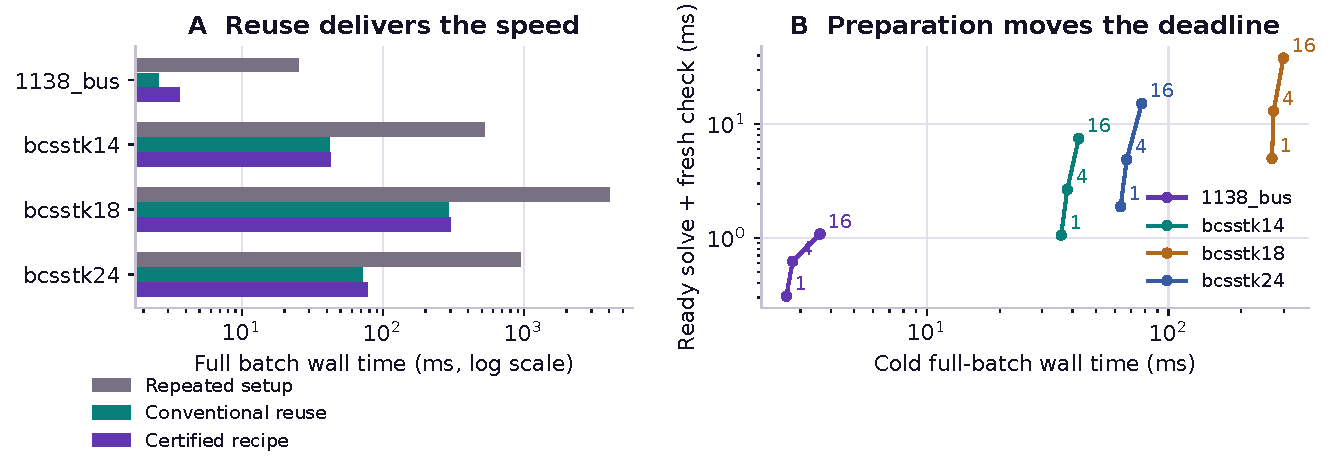
\includegraphics[width=\linewidth]{figures/readiness_frontier.pdf}
\caption{\obs{}. (A) Primary-count full-batch medians. (B) Certified full-batch cost versus ready solve-and-check latency; point labels are right-hand-side counts 1, 4 and 16. Connecting lines guide the eye between tested counts only. Both factors and synthetic right-hand sides exist at the ready-stage origin. Preparation is paid.}
\label{fig:frontier}\end{figure}

An independently written numerical checker recomputed 24 saved solution columns using explicit CSR sums and checked the logged criteria, source/data identities and accounting partitions across the full result ledger. Its supplemental audit passed 11,988 checks. This is implementation independence within the same research workflow, not independent institutional certification. The bounded CG diagnostic did not qualify on any of the four confirmation cases within 400 iterations; those results are retained rather than promoted as a new superiority claim over tuned iterative methods.

\subsection{Forecast skill resolves locally; adoption does not}
The preregistered primary deadline multiplier 1 yields Brier 0.072056 versus 0.259971 for the calibration-only pooled constant, across 720 correlated outcomes. The paired block interval for the score difference is $[-0.191480,-0.184338]$. Across all three deadline multipliers, the secondary score is 0.031463 versus 0.242373 on 2,160 correlated outcomes. The complete 180-target ledger was frozen before confirmation. Figure~\ref{fig:calibration} keeps these scopes separate.

The probabilities are not perfectly calibrated. Beta smoothing leaves the largest extreme bins underconfident, and intermediate bins are small. Conditioning on method, deadline and readiness distinguishes largely easy and hard local timing events; the constant comparator is weak. The result supports H3 for this narrow target, without establishing forecast skill across hosts, future workloads, scientific adoption or the intelligence transition itself. No external accepted-delivery probability was issued or scored as a success.

\begin{figure}[ht]\centering
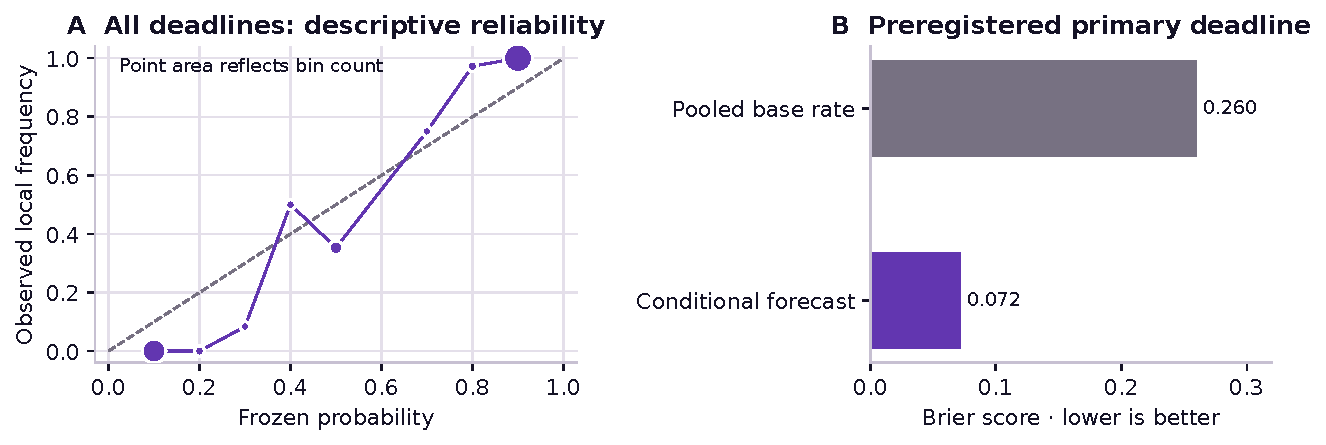
\includegraphics[width=\linewidth]{figures/calibration.pdf}
\caption{\obs{} outcomes of \pend{} forecasts issued before execution. (A) Descriptive reliability across all three declared deadline multipliers; correlated repeated targets and unequal bin counts limit interpretation. (B) Primary deadline score on 720 outcomes; the secondary all-deadline aggregate is shown separately. The baseline is a pooled calibration-only constant, not a specialist forecasting competitor.}
\label{fig:calibration}\end{figure}

\subsection{The timing policy does not establish unique net advantage}
The calibration-selected comparator is \texttt{static\_expert}, a fixed calibrated rule with permissible adaptive arrival recourse, not an observed human expert. The confirmation retains 32,256 policy rows over 4,608 paired worlds. An independently implemented audit reconstructs policy choices, probabilities, value of information, costs, block summaries and primary bootstrap intervals: 1,776,489 checks pass. It cannot reconstruct exact first-qualified timestamps that were not separately logged; it verifies the event bounds available in the retained fields.

\begin{figure}[ht]\centering
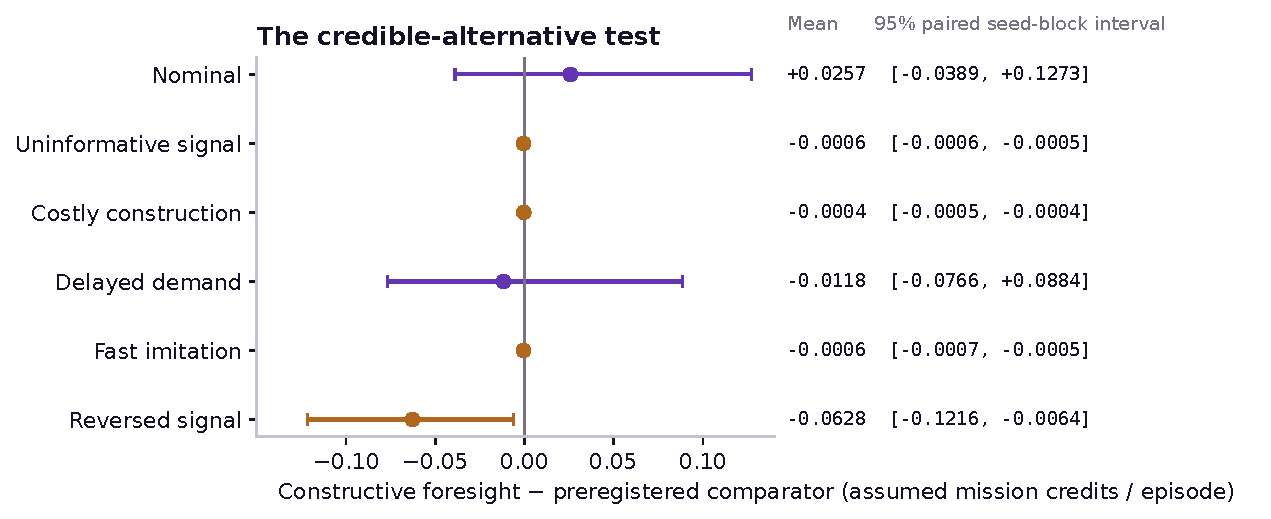
\includegraphics[width=\linewidth]{figures/causal_comparison.pdf}
\caption{\simu{}. Constructive foresight minus the locked calibrated fixed rule; one assumed credit per qualified on-time request and one credit per common clock unit of accounted cost. Intervals resample 24 complete seed blocks within each regime. They describe Monte Carlo variation under the stated model, not uncertainty about real markets or adoption. Tiny negative gaps in three regimes reflect extra controller work.}
\label{fig:causal}\end{figure}

The nominal effect is $+0.025667$ assumed credits per episode, with interval $[-0.038950,0.127277]$. The positive point estimate is too uncertain to establish the preregistered positive comparative claim. Delayed demand produces $-0.011762$ with an interval crossing zero. Reversed signal likelihood produces $-0.062780$, interval $[-0.121571,-0.006446]$. In the uninformative, costly-construction and fast-imitation regimes, native decisions and deliveries tie the fixed rule, while repeated deliberation adds small cost. H2 is therefore not established.

More decisively, the conventional compiled same-information policy has zero action disagreements with constructive foresight across all 4,608 worlds. Mean accepted counts are identical in every regime, while mean controller cost is lower. Its equal-regime advantage over constructive foresight is 0.000548 assumed credits per episode, interval $[0.000534,0.000565]$. This is a small computational efficiency difference, not an economic windfall. Equal information and an equally capable builder eliminate a unique-policy advantage claim in this tested model.

Constructive foresight does outperform the deliberately limited forecast-only and wait-then-build policies in the equal-weight descriptive aggregate. That contrast shows why these weak ablations are insufficient as the sole evidence for advantage. Appendix~\ref{app:comparisons} reports all eligible-comparator differences. No regime weighting was learned from confirmation; equal weighting is an analytic summary, not an estimate of industry prevalence.

The uninformative-signal control leads constructive foresight to buy no signal. Nominal acquisition occurs in 15.23\% of episodes. When a signal cannot change the best feasible action, its acquisition cost has no decision benefit. Eighty late attempts remain in the complete policy ledger with their consumed work charged; latent future service durations are never available to admission decisions. A forecast that becomes false after distribution change is retained as a failed prediction, not rewritten as a successful intervention.

\begin{figure}[ht]\centering
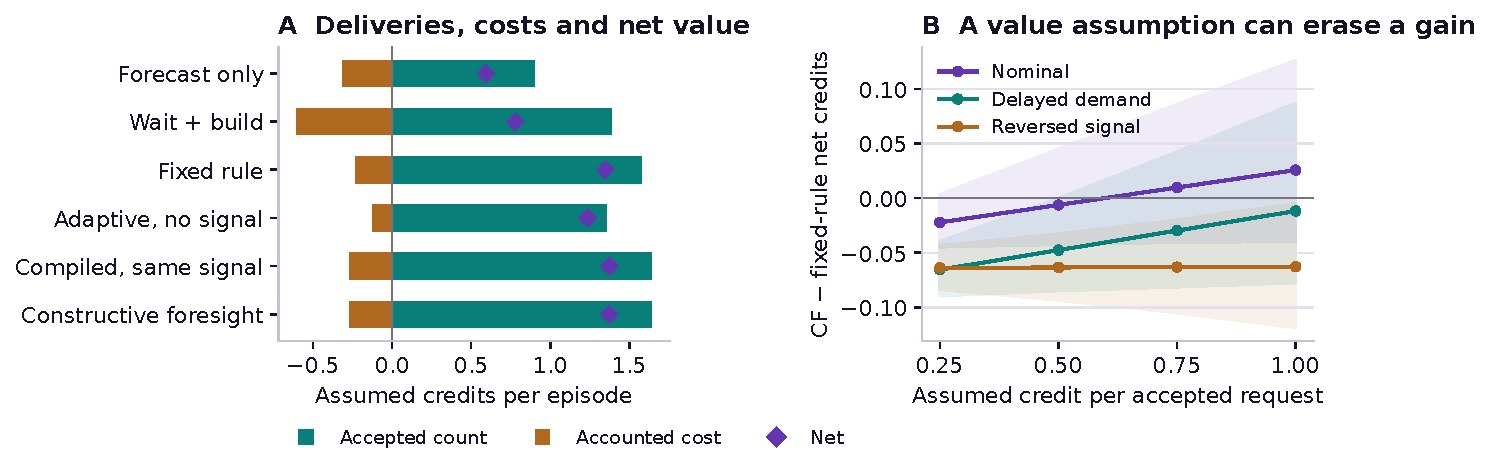
\includegraphics[width=\linewidth]{figures/value_decomposition.pdf}
\caption{\simu{} and \assum{}. (A) Nominal accepted counts, modeled accounted costs and net credits. Numerical wall times, assumed signal/competitor time and measured controller/preparation CPU use one explicit credit rate; they are not dollars or a measured CPU total. (B) Exploratory post-confirmation accounting sensitivity on the same fixed actions and outcomes: reducing assumed service value can erase the nominal gain. Shaded intervals are paired seed-block intervals; this is not a demand-elasticity or market-price forecast.}
\label{fig:value}\end{figure}

\subsection{Restoration works; permission and overhead remain real}
The fixed native demonstration completes initial construction and actual recipe restoration on 1138\_bus with four manufactured right-hand sides. Both outputs pass the separate checker. Restoration preserves parent lineage while returning no active authority, no current proof and no enabled execution. Fresh checking and a separate explicit public-fixture grant are required for the second inspection. Eight native refusal probes and six receiver refusals have the expected outcomes. The corrupted-output negative control fails proof before admission. These observations support H4 only for the tested published paths and fixture.

The complete native process costs 6.552 seconds wall and 6.427 seconds child CPU. Inside the two runs, orchestration and retention consume 2.392 and 3.156 seconds; their numerical handlers take 0.0093 and 0.0063 seconds. Provenance is not free. For kernels this small, a full lifecycle transaction around every solve would dominate useful work. Batching evidence at a justified capability boundary is a plausible engineering improvement, not a measured gain claimed by this study.

\begin{figure}[ht]\centering
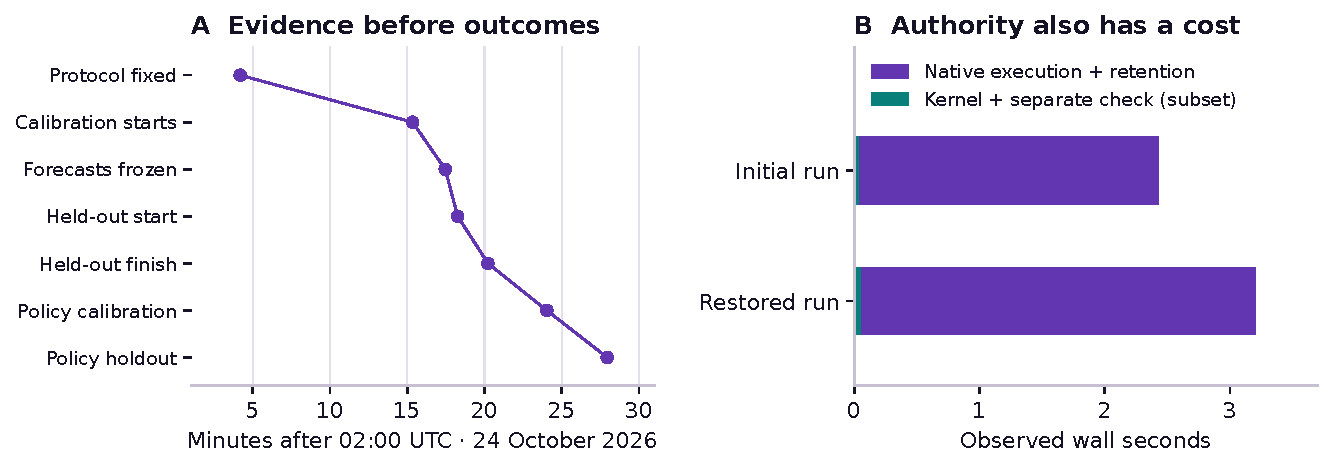
\includegraphics[width=\linewidth]{figures/decision_timeline.pdf}
\caption{\obs{}. (A) Retained protocol, calibration, freeze and confirmation timestamps in UTC document that forecasts preceded execution under the retained hashes. (B) Actual initial and restored native runs; the small colored subsets are numerical handler plus separate checking. The full process also includes startup and bridge work. These are local test-identity executions with no settlement or external authority.}
\label{fig:timeline}\end{figure}

\subsection{The full-cost verdict remains bounded}
The campaign measured 78.516 CPU seconds in numerical calibration and 117.283 in confirmation. The development serialization failure leaves a 9.948-second lower bound for completed batch CPU rather than a complete phase total. Decision calibration and confirmation consume 1.360 and 3.928 child CPU seconds; their policy-model preparation is not a free input to deployed model-using policies. Separate audits and the native process have their own ledger rows. Failure work is retained; validation and late-work subsets are never added twice.

Authoring inference charges, human review, maintenance, external acceptance and opportunity cost are unmetered. These entries are \emph{unknown}, not zero. No live payment, financial transaction, gas use or settled revenue occurred in this study; the hosting/platform charge is not independently known. A firm offer or willingness-to-pay observation is also absent. Consequently, the results establish numerical capability and a bounded model comparison, not positive full-cost commercial Mission Alpha. The detailed ledger retains native time units and makes no token-price or investment-return conversion.

\FloatBarrier
\section{Discussion: make readiness earn its cost}
\subsection{What the intelligence-transition question becomes}
The motivating question is deliberately large. The answer is useful only after becoming small enough to test: whose bottleneck, what output, which deadline, what proof, which alternative and at what total cost? Sector scale alone supplies none of those quantities. The audited macro envelope cannot decide whether a single solver should be prepared today.

The experiment demonstrates a practical distinction between \emph{capacity} and \emph{readiness}. A solver available from a library can solve the system; a retained factorization and known verification recipe can respond sooner to a repeated request. That change in readiness has an observed latency consequence. Yet the mechanism is available to a conventional engineer. Comparing only against repeated setup would overstate the contribution of foresight and of the certification wrapper.

The same lesson appears at the policy layer. Information can matter near a build threshold, but it is not valuable merely because it sharpens a probability. In the uninformative regime the policy correctly declines acquisition. In the nominal regime its uncertain gain over a fixed rule does not survive the stronger claim that the proposed procedure is uniquely better: a conventional compiled rule makes identical decisions. The positive candidate mechanism is therefore ordinary preparation plus decision-relevant information, deployed efficiently. The label \TI{} is a motivating discipline, not an additional source of measured value.

\subsection{Waiting, competition and distribution change}
Waiting has two different meanings in this study. Mandatory waiting followed by construction can miss a short deadline or buy an expensive capability too late. Adaptive waiting can preserve an option to use an alternative, build only when requests justify the cost, or decline unproductive work. A credible alternative must retain those choices. The better performance of adaptive policies over the wait-then-build ablation is not a finding that patience is irrational.

Imitation removes exclusivity before it removes usefulness. When competing capability becomes cheaply accessible, a beneficiary can gain even as the original builder loses an appropriable advantage. Fast imitation therefore improves available service routes in the model; it does not retroactively erase already delivered utility. Price compression is represented only through an explicitly labeled fixed-trajectory value sensitivity. The experiment does not estimate a market-clearing price, demand elasticity, monopoly duration or investor return.

The reversed-signal regime gives a more direct warning. A model can continue to produce coherent posterior decisions after its likelihood assumptions become wrong. In this case the nominally informative intervention reduces modeled net value. The response is not to reinterpret the loss as hidden success. It is to monitor the validity of the information model, retain an alternative policy, and require new evidence before committing to a materially changed plan.

\subsection{The strongest useful method actually found}
For the tested numerical workloads, use conventional factor reuse with per-output checking. Retain a source-bound reconstruction recipe when auditability and later restoration are needed. Preserve a calibrated delivery distribution that distinguishes already-paid preparation from a cold start. Use the simplest competent policy that implements the justified build, rent or wait decision, and charge its model preparation and execution. Require fresh capability evidence and separate authority when invoking a controlled action.

This recommendation is bounded to the measured instrument and finite model. It does not assert that compiled finite rules will dominate general agents on open-ended research. It does show what an agent must beat here. Repeating a deliberation that has already been compiled adds cost without changing the useful action. Wrapping a millisecond-scale kernel in seconds of lifecycle bookkeeping is also a poor default unless that bookkeeping buys a necessary assurance. Those are actionable engineering findings even when incremental commercial value is unknown.

\section{Limitations and the next decisive evidence}
The four matrices and manufactured inputs are a small benchmark, not a representative sample of scientific missions. Shared-host timing varies; there is no cross-machine or large-scale generalization result. Specialized Cholesky, tuned iterative methods and alternative orderings were not exhaustively compared. The bounded CG diagnostic is not a substitute for such a study. The instrument's known-solution error check is available in manufactured tests but generally unavailable for a novel physical problem.

The local forecasts resolve after issuance, but their deadlines are relative to known computational starts and often distinguish very easy from very hard conditions. The pooled constant is a limited reference. This is prospective local execution evidence, not a historical language-model backtest or a forecast of industrial adoption. Public matrices may already be known to language models, and assistant-assisted task design is not an independently blinded human selection process.

Demand, adoption, imitation, delay, amortization and mission-credit values are assumed. Model-conditional intervals do not cover uncertainty about those assumptions. The finite policy family cannot stand in for every competent organization. Native role separation uses a public shared test identity, not authentic independent actors. Fleet execution, physical instrumentation, fresh mainnet state, live funding and transaction behavior are outside the demonstrated boundary. Contract source continuity does not prove deployed-state continuity.

The cost ledger is auditable where measurements exist and explicitly incomplete elsewhere. A positive operational difference would still need to pay authoring, acquisition, engineering, review, maintenance, adoption and opportunity costs. No recruited beneficiary, accepted public pilot or payment receipt closes that gap. The original seven- and thirty-day adoption targets remain unmeasured; they are not generated as synthetic successes, and the paper does not score a future outcome before it occurs.

The next decisive study would recruit a numerical-research beneficiary, freeze a real workload and acceptance predicate, and prospectively assign comparable tasks to the readiness procedure and a competent conventional workflow. Both sides would receive the same tools and information budget; engineering and review effort would be independently recorded. The outcome would be accepted investigations delivered by a real deadline, with maintenance and full labor accounted for. That extension is a proposal, not part of the reported evidence, and no outreach or deployment is implied.

\section{Conclusion}
Could the intelligence transition be an extraordinary opportunity? It could. This study does not measure its total size or forecast which sector wins first. It identifies a more demanding unit of progress: an accepted capability that is ready in time and worth its full cost relative to a credible response.

The numerical artifact works. Its local delivery forecasts are testable and show skill. Its restoration and authority boundaries can be inspected and exercised. But the comparative study does not establish a unique full-cost advantage for constructive foresight: conventional reuse explains the numerical gain, and an equally informed compiled policy matches the decisions with less overhead. That boundary is the result, not a defect to hide.

\begin{claimbox}
\textbf{Build the capability. Prove the delivery. Make readiness earn its cost.}\\[3pt]
Useful foresight ends in a qualified action---including the decision to wait---whose incremental value survives a serious alternative.
\end{claimbox}


\clearpage

\begin{thebibliography}{28}
\providecommand{\natexlab}[1]{#1}
\providecommand{\url}[1]{\texttt{#1}}
\expandafter\ifx\csname urlstyle\endcsname\relax
  \providecommand{\doi}[1]{doi: #1}\else
  \providecommand{\doi}{doi: \begingroup \urlstyle{rm}\Url}\fi

\bibitem[Brier(1950)]{brier1950}
Glenn~W. Brier.
\newblock Verification of forecasts expressed in terms of probability.
\newblock \emph{Monthly Weather Review}, 78\penalty0 (1):\penalty0 1--3, 1950.
\newblock \doi{10.1175/1520-0493(1950)078<0001:VOFEIT>2.0.CO;2}.
\newblock URL
  \url{https://journals.ametsoc.org/view/journals/mwre/78/1/1520-0493_1950_078_0001_vofeit_2_0_co_2.xml}.

\bibitem[Davis and Hu(2011)]{davis2011}
Timothy~A. Davis and Yifan Hu.
\newblock The university of florida sparse matrix collection.
\newblock \emph{ACM Transactions on Mathematical Software}, 38\penalty0
  (1):\penalty0 1:1--1:25, 2011.
\newblock \doi{10.1145/2049662.2049663}.
\newblock URL \url{https://sparse.tamu.edu/about}.

\bibitem[Elmachtoub and Grigas(2022)]{elmachtoub2022}
Adam~N. Elmachtoub and Paul Grigas.
\newblock Smart ``predict, then optimize''.
\newblock \emph{Management Science}, 68\penalty0 (1):\penalty0 9--26, 2022.
\newblock \doi{10.1287/mnsc.2020.3922}.
\newblock URL \url{https://arxiv.org/abs/1710.08005}.

\bibitem[Gneiting and Raftery(2007)]{gneiting2007}
Tilmann Gneiting and Adrian~E. Raftery.
\newblock Strictly proper scoring rules, prediction, and estimation.
\newblock \emph{Journal of the American Statistical Association}, 102\penalty0
  (477):\penalty0 359--378, 2007.
\newblock \doi{10.1198/016214506000001437}.
\newblock URL
  \url{https://sites.stat.washington.edu/people/raftery/Research/PDF/Gneiting2007jasa.pdf}.

\bibitem[Hestenes and Stiefel(1952)]{hestenes1952}
Magnus~R. Hestenes and Eduard Stiefel.
\newblock Methods of conjugate gradients for solving linear systems.
\newblock \emph{Journal of Research of the National Bureau of Standards},
  49\penalty0 (6):\penalty0 409--436, 1952.
\newblock \doi{10.6028/jres.049.044}.
\newblock URL
  \url{https://nvlpubs.nist.gov/nistpubs/jres/049/jresv49n6p409_A1b.pdf}.

\bibitem[Higham(2002)]{higham2002}
Nicholas~J. Higham.
\newblock \emph{Accuracy and Stability of Numerical Algorithms}.
\newblock SIAM, 2 edition, 2002.
\newblock \doi{10.1137/1.9780898718027}.
\newblock URL \url{https://epubs.siam.org/doi/10.1137/1.9780898718027.ch7}.

\bibitem[Howard(1966)]{howard1966}
Ronald~A. Howard.
\newblock Information value theory.
\newblock \emph{IEEE Transactions on Systems Science and Cybernetics},
  2\penalty0 (1):\penalty0 22--26, 1966.
\newblock \doi{10.1109/TSSC.1966.300074}.
\newblock URL \url{https://ieeexplore.ieee.org/document/4082064/}.

\bibitem[Josefsson and Liusvaara(2017)]{rfc8032}
Simon Josefsson and Ilari Liusvaara.
\newblock Edwards-curve digital signature algorithm (eddsa).
\newblock RFC 8032, 2017.
\newblock URL \url{https://www.rfc-editor.org/rfc/rfc8032#section-7.1}.
\newblock Section 7.1, TEST 1: public test-vector keypair only.

\bibitem[Kolodziej et~al.(2019)Kolodziej, Aznaveh, Bullock, David, Davis,
  Henderson, Hu, and Sandstrom]{kolodziej2019}
Scott~P. Kolodziej, Mohsen Aznaveh, Matthew Bullock, Jarrett David, Timothy~A.
  Davis, Matthew Henderson, Yifan Hu, and Read Sandstrom.
\newblock The suitesparse matrix collection website interface.
\newblock \emph{Journal of Open Source Software}, 4\penalty0 (35):\penalty0
  1244, 2019.
\newblock \doi{10.21105/joss.01244}.
\newblock URL \url{https://joss.theoj.org/papers/10.21105/joss.01244}.

\bibitem[McDonald and Siegel(1986)]{mcdonald1986}
Robert McDonald and Daniel Siegel.
\newblock The value of waiting to invest.
\newblock \emph{The Quarterly Journal of Economics}, 101\penalty0 (4):\penalty0
  707--727, 1986.
\newblock \doi{10.2307/1884175}.
\newblock URL \url{https://doi.org/10.2307/1884175}.

\bibitem[{MONTREAL.AI}(2026{\natexlab{a}})]{alphaSource2026}
{MONTREAL.AI}.
\newblock Published successor runtime and ascension contract source,
  2026{\natexlab{a}}.
\newblock URL
  \url{https://github.com/MontrealAI/AGI-Alpha-Agent-v0/tree/dfc79c4ae81ac612cbff9865a0af8389b6ff3de9}.
\newblock Immutable Alpha source dfc79c4ae81ac612cbff9865a0af8389b6ff3de9.

\bibitem[{MONTREAL.AI}(2026{\natexlab{b}})]{atlas2026}
{MONTREAL.AI}.
\newblock Insight atlas field guide, 2026{\natexlab{b}}.
\newblock URL
  \url{https://github.com/MontrealAI/AGI-Alpha-Agent-v0/blob/dfc79c4ae81ac612cbff9865a0af8389b6ff3de9/docs/agent/INSIGHT_ATLAS.md}.
\newblock Source inspected at commit dfc79c4ae81ac612cbff9865a0af8389b6ff3de9;
  accessed 24 October 2026 UTC.

\bibitem[{MONTREAL.AI}(2026{\natexlab{c}})]{fleetSource2026}
{MONTREAL.AI}.
\newblock Agi fleet linux source, 2026{\natexlab{c}}.
\newblock URL
  \url{https://github.com/MontrealAI/AGI-Fleet-Linux/tree/45759fb096faf8988f58ae5ea71248d0f35a97c7}.
\newblock Immutable source 45759fb096faf8988f58ae5ea71248d0f35a97c7.

\bibitem[{MONTREAL.AI}(2026{\natexlab{d}})]{jobsSource2026}
{MONTREAL.AI}.
\newblock Agi jobs v0 source, 2026{\natexlab{d}}.
\newblock URL
  \url{https://github.com/MontrealAI/AGIJobsv0/tree/9983478d42c32fe399f28dd9b0e0173f904b8a11}.
\newblock Immutable source 9983478d42c32fe399f28dd9b0e0173f904b8a11.

\bibitem[{MONTREAL.AI}(2026{\natexlab{e}})]{mainnet2026}
{MONTREAL.AI}.
\newblock Current mainnet deployment record, 2026{\natexlab{e}}.
\newblock URL
  \url{https://github.com/MontrealAI/AGI-Alpha-Agent-v0/blob/dfc79c4ae81ac612cbff9865a0af8389b6ff3de9/docs/agent/CURRENT_MAINNET_DEPLOYMENT.md}.
\newblock Point-in-time record, not fresh chain verification; source at
  dfc79c4.

\bibitem[{MONTREAL.AI}(2026{\natexlab{f}})]{managerSource2026}
{MONTREAL.AI}.
\newblock Agi job manager source, 2026{\natexlab{f}}.
\newblock URL
  \url{https://github.com/MontrealAI/AGIJobManager/tree/c5958eae872458c2f3cac48fea0b4bbfadc6ac6c}.
\newblock Immutable source c5958eae872458c2f3cac48fea0b4bbfadc6ac6c.

\bibitem[{MONTREAL.AI}(2026{\natexlab{g}})]{outexecute2026}
{MONTREAL.AI}.
\newblock Out-execute, 2026{\natexlab{g}}.
\newblock URL
  \url{https://github.com/MontrealAI/AGI-Alpha-Agent-v0/blob/dfc79c4ae81ac612cbff9865a0af8389b6ff3de9/docs/Out_Execute.tex}.
\newblock Current source manuscript inspected at Alpha commit dfc79c4.

\bibitem[{MONTREAL.AI}(2026{\natexlab{h}})]{outlearn2026}
{MONTREAL.AI}.
\newblock Out-learn, 2026{\natexlab{h}}.
\newblock URL
  \url{https://github.com/MontrealAI/AGI-Alpha-Agent-v0/blob/dfc79c4ae81ac612cbff9865a0af8389b6ff3de9/docs/Out_Learn.tex}.
\newblock Current source manuscript inspected at Alpha commit dfc79c4.

\bibitem[{MONTREAL.AI}(2026{\natexlab{i}})]{outstrategise2026}
{MONTREAL.AI}.
\newblock Out-strategise, 2026{\natexlab{i}}.
\newblock URL
  \url{https://github.com/MontrealAI/AGI-Alpha-Agent-v0/blob/dfc79c4ae81ac612cbff9865a0af8389b6ff3de9/docs/Out_Strategise.tex}.
\newblock Current source manuscript inspected at Alpha commit dfc79c4.

\bibitem[{MONTREAL.AI}(2026{\natexlab{j}})]{registration2026}
{MONTREAL.AI}.
\newblock Writer 9 initial pre-experiment registration, 2026{\natexlab{j}}.
\newblock URL
  \url{https://github.com/MontrealAI/AGI-Alpha-Agent-v0/issues/4850#issuecomment-6378545862}.
\newblock Public coordination comment 6378545862; initial protocol and durable
  checkpoint hashes.

\bibitem[{MONTREAL.AI}(2026{\natexlab{k}})]{ti2026}
{MONTREAL.AI}.
\newblock Transformational intelligence, 2026{\natexlab{k}}.
\newblock URL
  \url{https://github.com/MontrealAI/AGI-Alpha-Agent-v0/blob/dfc79c4ae81ac612cbff9865a0af8389b6ff3de9/docs/Transformational_Intelligence.tex}.
\newblock Current source manuscript inspected at Alpha commit dfc79c4.

\bibitem[{MONTREAL.AI}(2026{\natexlab{l}})]{treasure2026}
{MONTREAL.AI}.
\newblock Living treasure map: illustrative envelope and horizon controls,
  2026{\natexlab{l}}.
\newblock URL
  \url{https://github.com/MontrealAI/MontrealAI.github.io/blob/2bd71648d0bb3cc752d7b36a899dece8ce6d243e/goalos-v67-alpha-agi-insight-living-treasure-map-masterclass-interface.html}.
\newblock Pinned source 2bd71648d0bb3cc752d7b36a899dece8ce6d243e.

\bibitem[Murphy(1993)]{murphy1993}
Allan~H. Murphy.
\newblock What is a good forecast? an essay on the nature of goodness in
  weather forecasting.
\newblock \emph{Weather and Forecasting}, 8\penalty0 (2):\penalty0 281--293,
  1993.
\newblock URL
  \url{https://journals.ametsoc.org/view/journals/wefo/8/2/1520-0434_1993_008_0281_wiagfa_2_0_co_2.xml}.

\bibitem[Parks et~al.(2006)Parks, de~Sturler, Mackey, Johnson, and
  Maiti]{parks2006}
Michael~L. Parks, Eric de~Sturler, Greg Mackey, Duane~D. Johnson, and Spandan
  Maiti.
\newblock Recycling krylov subspaces for sequences of linear systems.
\newblock \emph{SIAM Journal on Scientific Computing}, 28\penalty0
  (5):\penalty0 1651--1674, 2006.
\newblock \doi{10.1137/040607277}.
\newblock URL
  \url{https://personal.math.vt.edu/sturler/publications/SISC_KrylovRecycling_2006.pdf}.

\bibitem[Perdomo et~al.(2020)Perdomo, Zrnic, Mendler-D{\"u}nner, and
  Hardt]{perdomo2020}
Juan Perdomo, Tijana Zrnic, Celestine Mendler-D{\"u}nner, and Moritz Hardt.
\newblock Performative prediction.
\newblock In \emph{Proceedings of the 37th International Conference on Machine
  Learning}, volume 119 of \emph{Proceedings of Machine Learning Research},
  pages 7599--7609, 2020.
\newblock URL \url{https://proceedings.mlr.press/v119/perdomo20a.html}.

\bibitem[Purohit et~al.(2018)Purohit, Svitkina, and Kumar]{purohit2018}
Manish Purohit, Zoya Svitkina, and Ravi Kumar.
\newblock Improving online algorithms via {ML} predictions.
\newblock In \emph{Advances in Neural Information Processing Systems},
  volume~31, 2018.
\newblock URL
  \url{https://proceedings.neurips.cc/paper/2018/hash/73a427badebe0e32caa2e1fc7530b7f3-Abstract.html}.

\bibitem[Rubin(1974)]{rubin1974}
Donald~B. Rubin.
\newblock Estimating causal effects of treatments in randomized and
  nonrandomized studies.
\newblock \emph{Journal of Educational Psychology}, 66\penalty0 (5):\penalty0
  688--701, 1974.
\newblock \doi{10.1037/h0037350}.
\newblock URL
  \url{https://dash.harvard.edu/entities/publication/73120378-82c0-6bd4-e053-0100007fdf3b}.

\bibitem[{SciPy contributors}(2026)]{scipySplu}
{SciPy contributors}.
\newblock scipy.sparse.linalg.splu, 2026.
\newblock URL
  \url{https://docs.scipy.org/doc/scipy-1.17.0/reference/generated/scipy.sparse.linalg.splu.html}.
\newblock Installed experiment version 1.17.0; SuperLU CSC factorization and
  reusable solve interface.

\end{thebibliography}

\clearpage
\appendix
\section{Reproduction and evidence custody}\label{app:reproduction}
The complete source archive is the canonical research object. Its payload manifest identifies every source file, input, result, figure and authoritative PDF by SHA-256 and byte count. The PDF inside the archive is authoritative if a standalone document service attaches provenance or otherwise changes its bytes. A separately rebuilt PDF may differ in metadata while preserving the rendered research; the build verification records its outcome explicitly.

\begin{table}[ht]\centering\small
\begin{tabularx}{\linewidth}{@{}L{45mm}Y@{}}\toprule
Entry point & Purpose \\\midrule
\texttt{README.md} & Environment, exact commands, source pins and interpretation boundaries. \\
\texttt{protocol.json} / \texttt{amendments/} & Original hypotheses, fixed task selection, budget, information cutoffs and disclosed corrections. \\
\texttt{numerics.py} / \texttt{data/} & Frozen numerical instrument and exact pinned public inputs; no network fetch needed for execution. \\
\texttt{decision.py} / \texttt{decision\_protocol.json} & Frozen finite timing model and complete assumed distributions. \\
\texttt{results/} & Development, calibration, freezes and complete confirmation outcomes; adverse outcomes retained. \\
\texttt{check\_results.py} / \texttt{check\_decision.py} & Separate implementations of arithmetic, provenance, quality and accounting checks. \\
\texttt{demo\_harness.py} / \texttt{vendored/} & Bounded native lifecycle demonstration and exact unchanged source closure. \\
\texttt{COST\_LEDGER.json} & Measured runtime, failures and unknown cost categories without a fictional monetary total. \\
\texttt{make\_figures.py} / \texttt{paper/} & Original vector figures, complete LaTeX, bibliography and generated result tables. \\
\texttt{publication/} & Passive paper/source handoff; publication status is separate from research acceptance. \\\bottomrule
\end{tabularx}
\caption{\source{} and retained research outputs. File names describe inspectable entry points; they do not imply live deployment.}
\end{table}

The measured environment used Python 3.12.14, NumPy 2.3.5, SciPy 1.17.0 and threadpoolctl 3.6.0 with a single BLAS thread. Figures used Matplotlib 3.10.8; the native demonstration also used Pydantic 2.14.0 and cryptography 50.0.2. Exact environment records, including runtime libraries and platform, accompany each numerical phase. Host contention, caches and numerical-library builds can change timings. Reproduction means regenerating the procedure and checking its numerical outputs, not promising identical milliseconds on another machine.

Research, code and manuscript preparation used an AI-assisted local workflow. Separate assistant-written checkers and source reviews improve implementation scrutiny; they do not constitute external peer review, a recruited expert evaluation or independent beneficiary acceptance. Owner review and qualified publication remain distinct gates.

Read-only auditing and paper reconstruction do not rerun the science. A fresh experimental replication must use a new isolated copy, regenerate calibration, issue a new forecast freeze, and execute its own held-out runs within the declared launch interval. The original forecast window has expired; changing its timestamps would falsify the original evidence. The package provides a command that prepares a fresh run tree while preserving the archived results.

The paper can be rebuilt offline with XeLaTeX, BibTeX and the supplied vector PDFs. The full \texttt{paper/} directory is the reproducible source; a convenience flattened TeX file still requires the packaged figure PDFs. No paid service, chain transaction, API key or operational credential is required for the local research demonstration. The existing public RFC 8032 test key is deliberately unsuitable for authentication.

\subsection{Retained failures and amendments}
A01 records unavailable official matrix downloads, the rejected pattern-only candidate, unchanged matrix selection, pinned mirrors, preflight seed separation, unavailable CHOLMOD and the bcsstk24 metadata disagreement. A02 makes numerical estimands and shared workload-generation accounting explicit. A03 records a JSON metadata serialization defect after all 36 development cells had finished; only metadata serialization changed. Development's batch CPU lower bound is retained rather than invented into a complete phase total. A04 corrects future-duration information leakage during engineering of the decision model: admission must use calibrated estimates and pay for actual late work. All decision calibration and confirmation occurred after that correction and source freeze.

Native engineering attempts also retain an unsupported enum failure and an incompatible decimal-string representation before the successful fixture. Those attempts are evidence of development cost and correction, not extra scientific samples. The corrupted-output proof failure is an intentional negative control. Ten additional post-confirmation functional controls check zero and NaN outputs, wrong matrix identity, stale source/library recipes, changed acceptance, unauthorized restoration envelopes and valid fresh reconstruction. All pass their explicitly expected outcomes, without changing any protected source or scientific input. These controls are engineering evidence, not additional confirmatory samples. Later arithmetic and manuscript checks may improve auditing or presentation, but cannot change the frozen execution sources, inputs or observed outcomes.

\section{The macro envelope remains an assumption}\label{app:macro}
Table~\ref{tab:macro} records the two distinct source weight sets. The original macro experience starts from an editable \$15 quadrillion envelope over twenty years, with a horizon control from 3 to 40 years. Its base weights can be redistributed by interactive objectives and pressures. The later Insight Atlas fixture uses exact integer basis points and a separate 120-minute agent-firm scheduling default. Neither set predicts sector output, investable returns or adoption dates. Verified economic value in the audited Atlas is zero. \citep{atlas2026,treasure2026}

\begin{table}[ht]\centering\small
\begin{tabular}{@{}lrr@{}}\toprule
Sector & Original base weight (\%) & Atlas fixture (\%)\\\midrule
Energy &15&13\\
Compute &12&12\\
Science &13&12\\
Health &11&11\\
Materials &9&9\\
Robotics &8&8\\
Finance &8&7\\
Climate &7&7\\
Machine labor &9&7\\
Infrastructure &4&6\\
Education &2&4\\
Governance &2&4\\\midrule
Total &100&100\\\bottomrule
\end{tabular}
\caption{\assum{} / \source{}. These weights allocate an assumed total. They are editable scenario inputs, not measured wealth, TAM, forecasts, capture probabilities or investment returns. The numerical and decision experiments do not use them.}
\label{tab:macro}\end{table}

\FloatBarrier
\section{Every credible comparator and the uncertainty boundary}\label{app:comparisons}
\begin{table}[ht]\centering\small
\begin{tabular}{@{}lrr@{}}\toprule
Comparator & CF minus comparator & 95\% paired seed-block interval\\\midrule
Adaptive without signal & $+0.029270$ & $[-0.031659,+0.100599]$\\
Compiled same-information rule & $-0.000548$ & $[-0.000565,-0.000534]$\\
Forecast-only ablation & $+0.442200$ & $[+0.318578,+0.570494]$\\
Calibrated fixed rule (primary) & $-0.008415$ & $[-0.030491,+0.018849]$\\
Wait-then-build ablation & $+0.880558$ & $[+0.762344,+1.010803]$\\
\bottomrule\end{tabular}
\caption{\simu{}. Equal-weight six-regime descriptive means in assumed mission credits per episode. The full result JSON reports every regime against every comparator. The calibrated fixed rule remains the preregistered primary comparator; the clairvoyant menu is excluded from credible alternatives. Intervals resample paired seed blocks, preserve shared worlds across regimes, and do not estimate external-beneficiary variation.}\end{table}

The frozen primary intervals use the original evaluator's bootstrap stream. This additional all-comparator report uses NumPy PCG64 seed 9001 and 2,000 resamples. Differences in interval endpoints caused by the resampling stream do not change the preregistered values. The service-value sensitivity was specified after confirmation and reuses the exact fixed trajectories at credits 1, 0.75, 0.5 and 0.25 per accepted request. It is explicitly exploratory and does not refit a policy or simulate new demand.

\FloatBarrier

\section{An evidence map for every headline claim}
\begin{longtable}{@{}L{37mm}L{24mm}L{94mm}@{}}
\toprule Claim & Class & Exact supporting boundary\\\midrule\endhead
Qualified repeated solves & Observed & 432 held-out batch records, 3,024 right-hand sides; fixed numerical predicate on manufactured inputs.\\
Reuse saves execution time & Observed & Paired randomized-order comparison against repeated setup on four matrices, one host. Cached LU is the strong comparator.\\
Delivery probabilities show skill & Prospective, then observed & Frozen local computational deadlines issued before confirmation; primary multiplier 1; correlated blocks. No industrial-adoption inference.\\
Timing can alter modeled delivery & Simulated & Same exogenous worlds replayed for all finite policies; actual adoption and demand unobserved.\\
Foresight has no established unique net gain & Simulated / inference & Nominal interval crosses zero; same-information conventional policy chooses identical actions with lower controller cost. Bounded to the tested policy class.\\
Restored knowledge grants no permission & Observed fixture & Unchanged native inspect/restore, empty authority, fresh proof and explicit grant, refused stale operations; public test identity.\\
Contracts support bounded plan states & Source-derived & Five exact source comparisons and recorded ABI identities; no fresh deployed-state or transaction claim.\\
Commercial value or future adoption & Unobserved / pending & No recruited beneficiary acceptance, payment, firm offer or willingness-to-pay evidence. Seven- and thirty-day targets remain unmeasured, not synthetic successes.\\
\bottomrule
\caption{Evidence classes are not interchangeable. A source audit, simulation, computational acceptance and real beneficiary acceptance answer different questions.}
\end{longtable}

\section{Publication is a separate acceptance gate}
The authorized repository and issue 4850 retain publication ownership and review coordination. The isolated research package and passive page are designed for a focused receiving pull request. A successful local build or a public source branch does not establish merge, release, Pages deployment or live-link acceptance. The handoff status records the current receiving base, required review and qualified publication gates. Existing research editions and owner-held runtime boundaries are preserved.

The five requested contracts were inspected because they constrain future funded missions, not because this numerical experiment needs a transaction. No financial action, new credential, security-setting change or paid infrastructure commitment was made. Knowledge, capability evidence and execution authority remain three separate things all the way from the local artifact to any future deployment.

\end{document}
